%LaTex cheat sheet template
\documentclass[10pt,a4paper,landscape]{article}

\usepackage{xfrac}
\usepackage[utf8]{inputenc}
\usepackage{amsmath}
\usepackage{amsfonts}
\usepackage{amssymb}
\usepackage{multicol}
\usepackage{geometry}
\usepackage{lipsum}
\usepackage{titlesec}
\usepackage[nodisplayskipstretch]{setspace}
\usepackage{enumitem}
\usepackage{wrapfig}
\usepackage{minted}
\usepackage{tabularx}
\usepackage{booktabs}

\usemintedstyle{perldoc}
\setminted{
    breaklines=true,
}

\geometry{a4paper, left=0mm, top=0mm, right=0mm, bottom=1mm}

\titlespacing{\section}{0pt}{0pt}{0pt}
\titlespacing{\subsection}{0pt}{0pt}{0pt}
\titlespacing{\subsubsection}{0pt}{0pt}{0pt}

\setlength{\abovedisplayskip}{0pt}
\setlength{\belowdisplayskip}{0pt}
\setlength{\parindent}{0pt}

\begin{document}
\begin{multicols*}{2}
    \section*{EmbHardw}
    \subsection*{Architecture}
\underline{Exemple de shéma d'architecture:}
\begin{enumerate}[topsep=0pt, partopsep=0pt, itemsep=0pt, parsep=0pt]
    \item Quand les données sont prêtes, I2S IN génère une IRQ
    \item Le processeur répond à l'IRQ en activant le DMA pour transferer les données vers la mémoire.
    \item Le processeur active le block FFT qui lis les données de la mémoire externe et génère une IRQ une fois la FFT terminée.
    \item Le processeur effectue ses calculs à parir des données venant du block FFT.
    \item Le processeur active le block iFFT qui les données du processeur et génère une IRQ une fois la iFFT terminée.
    \item Le processeur répond à l'IRQ en activant le DMA pour transfert de données vers la mémoire.
    \item I2S OUT génère une IRQ quand il est prêt à lire les données avec le DMA. Il lis les données et les envoie sur le bus I2S ensuite il génère une interrupttion une fois qu'il a fini.
\end{enumerate}
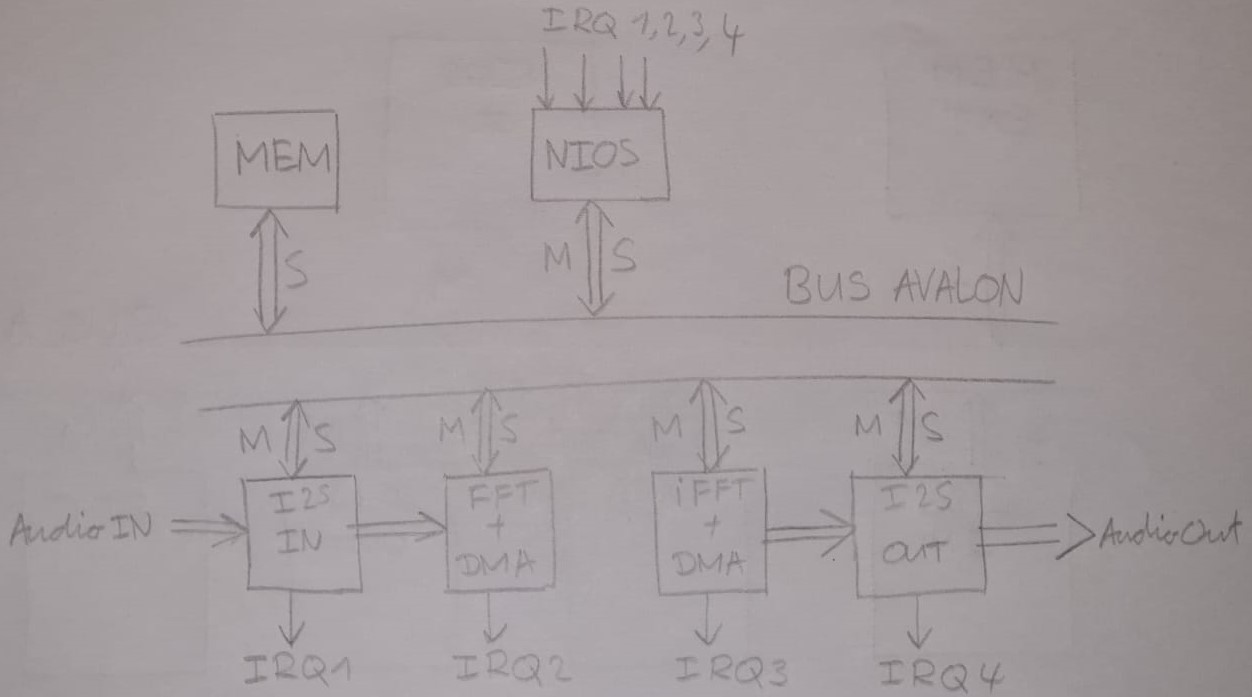
\includegraphics[width=\columnwidth]{images/schema_exa_ex1.jpg}
\underline{Exemple d'identity port:}
\begin{minted}{vhdl}
entity i2s_out is
    port (
        -- Avalon slave interface
        clock : in std_logic;
        reset : in std_logic;
        address : in std_logic_vector(1 downto 0);
        read : in std_logic;
        write : in std_logic;
        write_data : in std_logic_vector(31 downto 0);
        waitrequest : out std_logic;
        read_data : out std_logic_vector(31 downto 0);
        -- I2S interface for D/A
        sdim : out std_logic;
        lrclk : out std_logic;
        mclk : in std_logic;
        dem_sclk : in std_logic;
    );
end i2s_out;
\end{minted}

\underline{Exemple de modèle de registre:}

\begin{table}[H]
    \centering
    \begin{tabularx}{\columnwidth}{
            @{}
            >{\hsize=0.5\hsize}X % 1st column, 20% smaller
            >{\hsize=0.95\hsize}X % 2nd column, 20% smaller
            >{\hsize=0.95\hsize}X  % 3rd column, 20% smaller
            >{\hsize=0.4\hsize}X % 4th column, 20% smaller
            >{\hsize=2.05\hsize}X % 5th column, 80% larger
            @{}
        }
        \toprule
        Reg Address & Reg name C & Reg name VHDL & R/W & Description                                                                    \\
        \midrule
        1           & DATA       & dmaData       & W   & En soft pour passer les données brutes, en hard comme data input               \\
        2           & ADDR       & dmaAddr       & W   & Addresse à atteindre par le DMA                                                \\
        3           & SIZE       & dmaSize       & W   & Taille du mot à transmettre                                                    \\
        4           & STATUS     & dmaStatus     & W   & Dit si le DMA est libre                                                        \\
        5           & CONTROL    & control       & W   & 0 reset, 1 raw data, 2 channel when raw data or launch DMA, 3 anable interrupt \\
        6           & FREQ       & freq          & W   & Fréquence d'opération de la communication sérielle                             \\
        \bottomrule
    \end{tabularx}
\end{table}

\underline{Différence streaming et memory mapped:}\\
Le streaming permet de réduire la latence et la bandepassante nécessaire pour le transfert
car les datas peuvent être envoyées et reçues en continu. La méthode memory-mapped est plus
flexible et moins complexe à implémenter
    \subsection*{Hardware Software co-design}
\underline{Loop unrolling:}\\
Loop unrolling consits of replicating the body of a loop to reduce the number of iterations.

\begin{minipage}{0.69\columnwidth}
    \begin{minted}{c}
for (i = 0; i < 3; i++) {
    for (j = 0; j < 3; j++) {
        a[i][j] = 0;
    }
}
\end{minted}
\end{minipage}
%\hfill
$\Longleftrightarrow $
\begin{minipage}{0.29\columnwidth}
    \begin{minted}{c}
a[0][0] = 0;
a[0][1] = 0;
a[0][2] = 0;
a[1][0] = 0;
a[1][1] = 0;
a[1][2] = 0;
a[2][0] = 0;
a[2][1] = 0;
a[2][2] = 0;
\end{minted}
\end{minipage}

\underline{In-lining:}\\
In-lining consists of replacing a function call by the body of the function.
The keyword \texttt{inline} can also be used to force the compiler to inline a function.
The compiler option \texttt{-O3} enables in-lining.

\begin{minipage}{0.49\columnwidth}
    \begin{minted}{c}
int sum(int a, int b) {
    return a + b;
}
int main() {
    int a = 1;
    int b = 2;
    int c = sum(a, b);
    return 0;
}
\end{minted}
\end{minipage}
%\hfill
$\Longleftrightarrow $
\begin{minipage}{0.49\columnwidth}
    \begin{minted}{c}
int main() {
    int a = 1;
    int b = 2;
    int c = a + b;
    return 0;
}
\end{minted}
\end{minipage}
\underline{Using bit shift instead of multiplication/division:}\\
Multiplication and division are very expensive operations in terms of clock cycles.
It is therefore preferable to use bit shift when possible.

\begin{minipage}{0.49\columnwidth}
    \begin{minted}{c}
int main() {
    int a = 1;
    int b = 2;
    int c = a * b;
    return 0;
}
\end{minted}
\end{minipage}
%\hfill
$\Longleftrightarrow $
\begin{minipage}{0.49\columnwidth}
    \begin{minted}{c}
int main() {
    int a = 1;
    int b = 2;
    int c = a << 1;
    return 0;
}
\end{minted}
\end{minipage}
\underline{Computing inside the return statement:}\\

\begin{minipage}{0.49\columnwidth}
    \begin{minted}{c}
int main() {
    int a = 1;
    int b = 2;
    int c = a + b;
    return c;
}
\end{minted}
\end{minipage}
%\hfill
$\Longleftrightarrow $
\begin{minipage}{0.49\columnwidth}
    \begin{minted}{c}
int main() {
    int a = 1;
    int b = 2;
    return a + b;
}
\end{minted}
\end{minipage}

\underline{Eviter les accès mémoire:}

Par exemple rajouter des variables \texttt{*source} et \texttt{*dest} pour éviter les accès mémoire.

\begin{minipage}{0.49\columnwidth}
    \begin{minted}{c}
int r,g,b;
int x,y,index;
for (y = 0; y < 480; y++) {
    for (x = 0; x < 640; x++) {
        index = y * 640 + x;
        r = source[index];
        g = source[index + 1];
        b = source[index + 2];
    }
}
\end{minted}
\end{minipage}
$\Longleftrightarrow $
\begin{minipage}{0.49\columnwidth}
    \begin{minted}{c}
int r,g,b;
int x,y,index;
int *source;
int *dest;
for (y = 0; y < 480; y++) {
    for (x = 0; x < 640; x++) {
        index = y * 640 + x;
        r = *source++;
        g = *source++;
        b = *source++;
    }
}
\end{minted}
\end{minipage}

\columnbreak

\underline{Trade-off}

On peut remplacer certains bouts de code par du hardware en utilisant des
custom instructions.

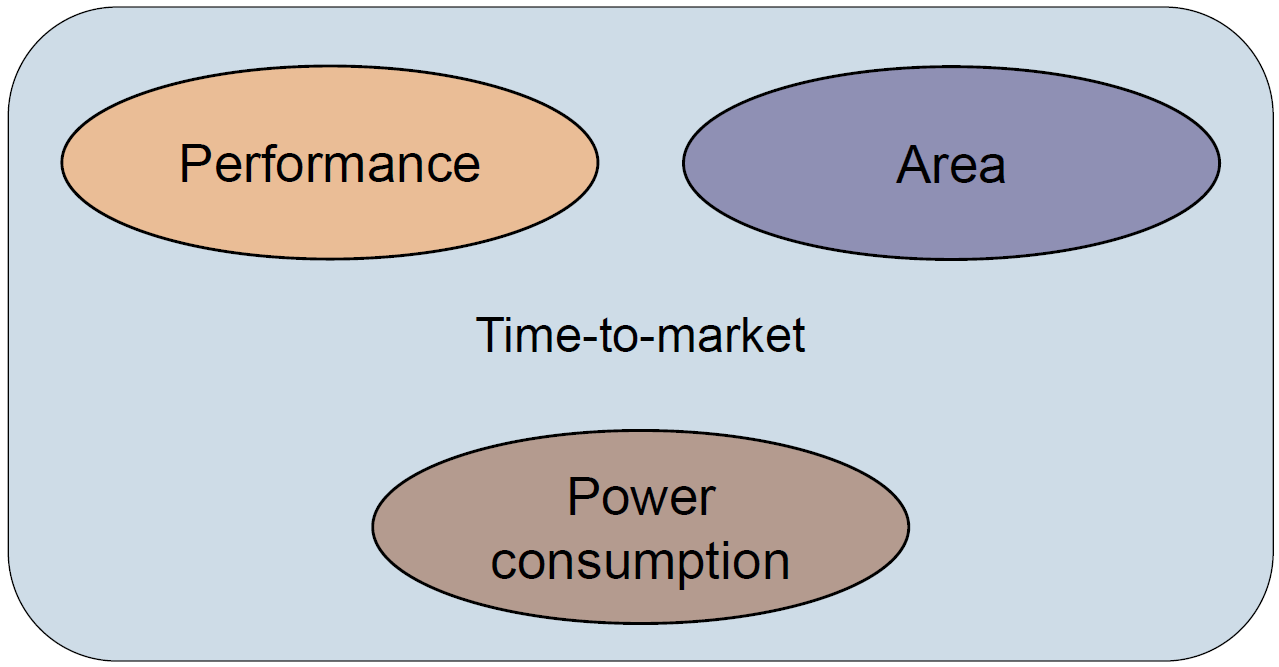
\includegraphics[width=\columnwidth]{images/trade_off_power_area_perf.png}
Facteurs limitants:
\begin{enumerate}[topsep=0pt, partopsep=0pt, itemsep=0pt, parsep=0pt]
    \item Compléxité de l'algorithme à remplacer
    \item Dispoinibilité de ressources hardware
    \item Temps de développement
\end{enumerate}
Avantages:
\begin{enumerate}[topsep=0pt, partopsep=0pt, itemsep=0pt, parsep=0pt]
    \item Performance accrue
    \item Consomation réduite
\end{enumerate}

\underline{Cache:}

Stocke les données les plus utilisées dans un espace mémoire plus rapide.

\underline{Scratchpad:}
Mémoire qui stock les données temporaires du processeur.

\underline{Problème de cohérence:}
Quand deux ou plusieurs processeurs essayent d'accéder à la même donnée en même temps.
Résultats imprévisibles.

MSI (Modified, Shared, Invalid) est un protocole de cohérence de cache.

Mutex: permet de bloquer l'accès à une ressource partagée.

\underline{Profiling:}
Méthode pour analyser les performances d'un programme. Avec un timer on compte le nombre
de cycles d'exécution d'une fonction. Il faut que le timer soit plus rapide que la fonction
qu'on étudie et il faut un timer hardware.



\end{multicols*}
\end{document}

\subsection*{Nios II}
\underline{NIOS II:}\\
a soft-core processor that can be implemented on Altera FPGA devices. It has a 32-bit RISC architecture and supports instruction and data caches, hardware multipliers, and custom instructions.\\
\underline{Avalon bus:}\\
a standard interface for connecting components in a SOPC. It supports different types of transfers, such as basic, burst, pipelined, and latency-tolerant. It also supports multiple masters and slaves, and provides signals for address, data, byte enable, wait request, and read data valid.\\
\underline{Embedded system on FPGA:}\\
are systems that integrates a NIOS II processor, memory, peripherals, and custom logic on a single FPGA chip. It has the advantages of fast implementation, modular architecture, affordable system complexity, reuse of existing IP cores, ease of development, and adaptability.

%NIOS II is a softcore processor from Altera that can be synthesized by a compiler and placed and routed on the FPGA. It has a 32-bit architecture with 256 instructions available for user implementation. There are three basic configurable architectures: Nios II/f, Nios II/s, and Nios II/e. The processor can be extended by user own instructions, up to 256. The ALU can be extended by custom user instructions, which can have access to all the FPGA resources. For cycles consuming operations, a hardware accelerator can be included/developed. The Avalon bus is a multi-master, synchronous bus that supports concurrent master-slave access. The ChipSelect is generated by the Avalon bus and selects the module. The Address[n .. 0] is used to access a specific register/memory position in the selected module. The Read and Write signals specified the direction of the transfers. They are provided by a Master and received by the slave modules. The direction is the view of the Master unit. The ReadData(..) and WriteData(..) bus transfers the Datas from (read)/ to (write) the Slaves. The master starts a transfer (read or write) and provides the Addresses (32 bits on NIOSII). It waits on WaitRequest signal to resume the transfer. Some positive points of a softcore architecture include fast implementation, modular architecture, affordable system complexity, good documentation, reuse of existing IP cores, ease of development of our own programmable interface on internal bus (i.e. Avalon in VHDL, Verilog), full system on FPGA, easily adaptable, and operating systems available. Some negative points include several complex tools to develop a system: hardware and software specific, and several debugging levels to deal with for hardware and software.

%This is a summary of a programmable parallel port interface design for an Avalon bus as a slave module. The module has a bidirectional port, programmable direction for each bit, and special features for modifying the port bits. The methodology for designing the interface includes identifying inputs-outputs of the interface, defining a register model, and creating the interface architecture. The parallel port module on Avalon has a bidirectional port, and the state value is stored in a register. There are three possible ways to modify the register value: RegPort, RegSet, and RegClr. The register can be read back. The internal signals for register access include iRegDir, iRegPort, and iRegPin. The architecture for the parallel port module includes registers access for write and read, and external interface for parallel port output value and input value.

%DMA stands for Direct Memory Access. It is a more efficient system for transferring data between the I/O and memory when the transfer rate is high. The transfer is carried out by a specialized unit called the DMA controller. The DMA controller performs transfers instead of the processor. DMA must have control of the bus as a Master including Address bus, Data bus and Control signals. The DMA controller is a programmable interface that must be programmed by the processor before it is operational. The DMA unit can be used to transfer data more efficiently than the processor. There are two main types of transfers: Memory to memory and Interface to memory (and vice versa). The DMA controller is a programmable interface. It must therefore be initialized prior to use. Several methods are possible depending on the circuit used: by direct access to internal DMA registers by the processor or by descriptors automatically loaded from memory to the DMA controller by itself. A minimum set of descriptors are available on virtually all DMA controllers: Source Address, Destination Address, Length of data to transfer, Modes of operation, Status of the controller, and Interrupt control.

